
%#############################################
\subsection{Introduction}
%#############################################
The literature about participatory budget is vast. The possibility of enhancing democracy through direct participation of citizens in a crucial political decision, i.e., budget allocation, attracted the attention of researches since the first well known experiences in Porto Alegre, in the 1980 decade.

Since then, several implementations all over the world were experimented, with many successful and fail stories. The use of online tools, both for supporting PB process and for publishing related datasets was also part of the more recent experiences.

In this review, we try to picture the state of art of PB, pros and cons and the mechanisms used, with a special focus on the online ones. The final objective is to detect how online information systems can help build a more effective participation, both higher and better informed, to produce better outcomes.

%#############################################
\subsection{Summary of Analysed of Works}
%#############################################
\begin{itemize}
	\item Origins of PB, and impact analysis in Brazil~\cite{Goncalves2014}
	\item Definitions: \cite{Zhang2013}
	\item Description of Cuiabá case: \cite{Borges2012}
	\item PB critics: \cite{Masser2013}
	\item 10 reasons to implement: \cite{Nitschke2013}
	\item Comparisson between online and offline PB: \cite{Peixoto2009}
	\item Conditions for participation: \cite{Addor2012}
	\item Budget data publishing process, including feedback: \cite{Alexopoulos2014}
	\item Deep analysis about PB, focusing on the poor \cite{TheWorldBank2001}
	\item Literature review, definitions and a model to analyse PB \cite{Miller2014}
\end{itemize}

As a complementary approach, we also interviewed two domain experts: 
\begin{itemize}
	\item a government employee who activeley supported a PB process
	\item and the director of a transparency oriented Civil Society Organization (CSO)
\end{itemize}

%#############################################
\subsection{Origins}
%#############################################

\cite{Goncalves2014} describes the first PB experiences in Brazil in the context of the country's redemocratization. After 20 years of military dictatorship, in the late 1980's, many efforts were driven in order to decentralize the public administration, from the federal level to the cities. In this context, the Workers Party was created, and as soon it elected the first mayors, PB was implemented as a symbol of direct democracy and transparency, as oposed to the previous regime.

Still according to \cite{Goncalves2014}, in Porto Alegre, the most cited PB showcase, the number of participants raised from around 1000, in 1989, to around 20,000 in the late 1990/early 2000. The alleged reason is that the people demands were realy undertaken by the governments.

According to \cite{Miller2014}, in 2010 nearly 1,500 municipalities worldwide adopted PB.

%#############################################
\subsection{PB Cycle}
%#############################################
According to~\cite{Giacomoni2007}, the classical Budget cycle comprises 4 phases:

\begin{enumerate}
\item Elaboration and presentation
\item Legislative authorization
\item Programming and execution
\item Evaluation and controll;
\end{enumerate}


Figure~\ref{fig:POA} shows the workflow used in Porto Alegre.

\begin{figure}[h]
\begin{center}
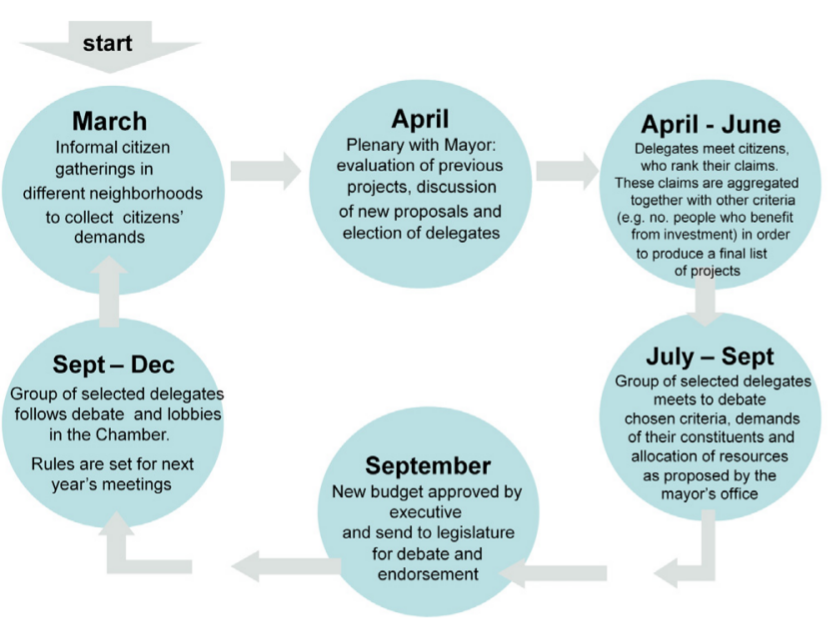
\includegraphics[scale=0.35]{images/portoalegreworkflow.png}
\caption{Workflow of Porto Alegre's PB. Author: \cite{Goncalves2014}\label{fig:POA}}
\end{center}
\end{figure}

\cite{TheWorldBank2001} summarizes four fases, illustrated in Figure~\ref{fig:WB}:
\begin{enumerate}
\item Budget formulation
\item Budge analysis
\item Budget expenditure
\item Performance monitoring
\end{enumerate}

\begin{figure}[h]
\begin{center}
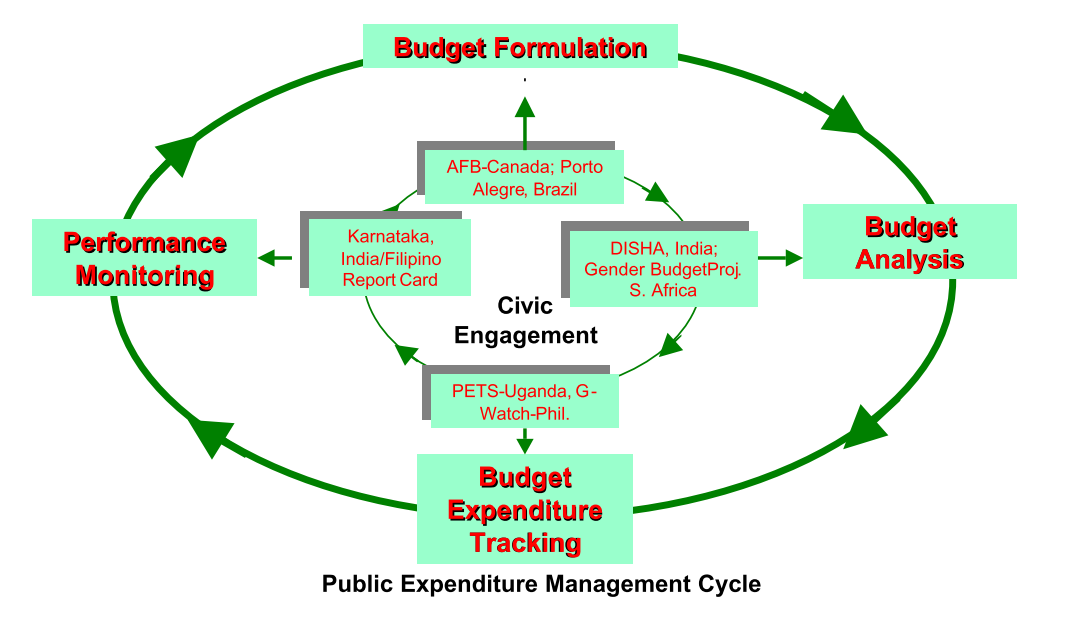
\includegraphics[scale=0.35]{images/cycle_WB.png}
\caption{Generic PB Workflow. Author: \cite{TheWorldBank2001}\label{fig:WB}}
\end{center}
\end{figure}



%#############################################
\subsection{Definitions}
%#############################################

\cite{Zhang2013} proposed some definitions on this field:

\noindent\textbf{Participatory budgeting} refers to a situation in which government officials invite citizens' input during the budget process and allows citizen to influence budgetary decisions (Zhang \& Yang, 2009).

\noindent\textbf{Mechanisms of participatory budgeting} refer to any tools provided by government for citizen involvement, including public hearings, citizen surveys, telephone hotlines, citizen advisory boards, focus group, as well as encouraging citizens to speak about budget in regular meetings, posting budget materials on the Internet, working with local media to highlight citizen comments during deliberation, and so on.

These mechanisms are of two kind:

\noindent\textbf{One way mechanisms:} Coordinating with the local media, such as TV and radio, to invite the public comments; Citizen surveys about spending priorities and needs through mail, Internet or telephone; Posting budget materials on Internet sites; Hotlines for citizens to provide suggestions or comments.

\noindent\textbf{Two way mechanisms:} Public budgetary hearings; Forums or workshops open to citizens during budget preparation; Opportunities for citizens to speak at regular meetings; Citizen advisory boards; Focus groups.
We define “two-way communication” as a process of face-to-face interaction between citizens and government officials in which citizens are provided with an opportunity to directly raise concerns and discuss them with government officials. Two-way communication can nurture social learning and collaborations between citizens and government because it enables stakeholders to respect and listen to one another’s opinions, and allows competing perspectives to be aired and considered before decisions are made (King, Feltey, \& Susel, 1998; Roberts, 2004).

In his review, \cite{Miller2014} also collected a number of other definitions. They also point some literature confusions, specially in the US. One of the points is that labelling the above mentioned one way mechanisms as PB ``eliminates from participatory budgeting what is distinctive, valuable, and potentially transformative".

%#############################################
\subsection{Motivations for implementing PB}
%#############################################

In a sort of ``marketing paper", \cite{Nitschke2013} proposes 10 reasons for public administrations to addopt PB:

\begin{enumerate}
\item Greater acceptance of priorities that are better harmonised
\item Making administration more efficient by integrating citizens’ knowledge
\item Increasing problem-solving capabilities
\item Greater cost awareness
\item Mobilising citizen engagement
\item Reducing political disenchantment and disillusionment with political parties
\item Fostering democracy
\item Supporting modernisation processes within the administration
\item Improved image for the local authority
\item Risks do exist, but they can be successfully managed
\end{enumerate}

As we will see in the next section, many of these ``benefits" can turn into impediments if not well implemented.

The political conditions for a sucessfull participation process are object of a political science oriented study by \cite{Addor2012}. After deeply analysing two experiences - not only of PB, but of wider participation practices - he formulated seven factors that influenced on the establishment and strengthening of the participator practices:

\begin{enumerate}
\item Politicisation of the society
\item Transformation of the reality
\item Permission of the utopia
\item Basis organization
\item Exchanges with other experiences
\item Involvement of the state
\item Formalization of the political commitment
\end{enumerate}

%#############################################
\subsection{Criticisms on PB}
%#############################################

\citeonline{Masser2013} summarized common criticisms to PB, specially in the German context. He considered that the first wave of PB experiences in the country failled: ``The original objective of involving citizens in the complex process of municipal budget formulation was not achieved, and has since been abandoned. Nowadays, it is only collections of proposals for measures and (investment) projects, or voting procedures on proposals made by policymakers and administrators, that operate under the label ‘participatory budgeting’."

The first argument is about \textbf{low participation}. ``The question therefore arises of whether the measures identified through PB possess sufficient legitimacy to warrant their adoption by democratically elected local councils."

This leads to a second argument that states the \textbf{under representation} of the society in PB practice.

Another argument lies in the \textbf{high cost of participation}, which is a consequence of the low participation. ``The low figures for participation raise another problem:  how sustainable is citizen participation through PB? In many cases we can see that PB has already been discontinued. The question as to whether ‘participatory budgeting’ as a whole is gradually fading away seems warranted. This is because, as with employee suggestion schemes, in PB fresh ideas are not forthcoming every day. In fact, there is a risk that the debate will keep returning to many similar proposals or even the same ones."

\textbf{Conclusions:}
The original intention of integrating citizens closely into the budget formulation process has not been realised;

The influence that citizens wield in this procedure is limited, because only a few proposals made by a few citizens have a chance of being realised, even though each and every citizen does have an opportunity to influence things by prioritising and voting on the proposals;

The fact that the influence of citizens is not all that significant might also benefit PB, in that members of local councils might then be far more willing to embrace this tool. 

There remains a trend toward PB. The Fifth Status Report on ‘Participatory Budgeting in Germany’ published in March 2012 identifies 21 newly active municipalities that are conducting PB. This makes a total of 115 active local authorities that are either conducting PB or have at least done so within the last two years.

%#############################################
\subsection{Some current PB cases}
%#############################################

\subsubsection{\href{http://pbnyc.org/}{New York}}
``New York City is experiencing a new kind of democracy. Through Participatory Budgeting, residents of twenty-four Council Districts across the City are directly deciding how to spend \$25 million of taxpayer money. From September 2014 to April 2015, community members are exchanging ideas, working together to turn ideas into project proposals, and voting to decide what proposals get funded."

\subsubsection{\href{http://cambridgema.nationbuilder.com}{Cambridge}}
``In December, community members shared over 380 ideas for projects to improve Cambridge.  From January-March, 40+ volunteer Budget Delegates prioritized and developed those ideas into 20 concrete project proposals for community members to vote on. Over 2,700 Cambridge residents age 12 and older voted online and at events around town from March 22-28, 2015 to decide which projects the City should fund."

\subsubsection{\href{https://budgetparticipatif.paris.fr}{Paris}}
In Paris, the major selected 15 projects and made \$20 million Euros for that. Over 40,000 people participated, being 40\% online. Among the 15, nine project were chosen to be developed in 2015. This year, almost 20,000 people proposed over 5,000 ideas.

\subsubsection{\href{http://planejasampa.prefeitura.sp.gov.br/}{São Paulo}}
In São Paulo, the Planning and Budget Participatory Cycle envisages a four year cycle, and is based on fisical goals. Direct participation resulted in 123 goals. 11,000 people formulated (physically) 9,489 suggestions, which resulted in the goals. There were also 2 hacker meetings, with 100 presential participants. A tool was developed for monitoring the goals by the elected councillors.

\subsubsection{Other related links}
\begin{itemize}
	\item \href{http://pbnetwork.org.uk/}{PB Network (UK)}
\end{itemize}

%#############################################
\subsection{Profile of the Participants}
%#############################################
\cite{Masser2013} reports that ``The vast majority are middle-aged men who left school well-qualified and now have well-paid jobs". 

On the other hand, \cite{Goncalves2014} reports that ``data collected at the participatory budgeting forums in Porto Alegre, in 2002, reveal that the participatory assemblies tend to concentrate a higher proportion of (i) women, (ii) elders and retired workers, (iii) married people, (iv) non-qualified workers, (v) people with lower average income, (vi) higher rates of associative life, and (vii) stronger identification with the Workers’ Party ideology than the city’s average dweller."

\cite{Peixoto2009} also reports advanced age and lower socio-economic background.


%#############################################
\subsection{The role of online tools in PB}
%#############################################
The use of online tools for PB was described by \cite{Peixoto2009}. According to him, ``evidence suggests that the online forum was, overall, an environment of rational, argumentative and reflective debates where active participants would persuade and be persuaded of the importance of one public work over another and where readers - in larger numbers - could be informed on concurrent perspectives."

In the voting for priorities, as expected, the participation was higher than the standard PB. It was noticed that people tend to vote locally, i.e., to choose works near their residences. This is also somehow expected, as the original target of PB is to descentralize power and let communities decide what is better for them.

``One element that was considered important for the success of the e-PB was the city’s communication campaign, which focused on the initiative and its novelty factor.''

Finally, the author considers that online PB should be just a complementary action to be taken together with tradiciontal PB. 


%#############################################
\subsection{Linking Budget Planning with final result}
%#############################################
As pointed by several works \cite{Addor2012, Miller2014, TheWorldBank2001, Borges2012}, a crucial element for raising participation is to guarantee that the decisions taken by the citizen council will be really implemented. Although this is a quite obvious conclusion, the disconnection between what is decided and what is implemented has been pointed to be the reason of several PB experiences (\cite{Borges2012}).

One of the interviewees was a government employee responsible for coordinating a PB process in a medium size city in Brazil. The process of collecting citizen demands was successful, with high participation of citizens and community leaders. All PB assemblies had the presence of at least four government representatives, so that proposals could be discussed with the ones responsible to implement it. 

However, the final result was modified by the legislative, and not totally implemented in the following year. In second year of PB, a new mayor was elected, and PB received less attention. The government officials stopped attending the meeting, and PB failed.

Another big issue pointed by the interviewee was the lack of transparency inside government. In his opinion, government information systems suffer from a lack of integration that seriously compromises transparency. With an integrated information approach, citizens could easily follow a demand from budget planning until the execution, and even assess specific targets, for example, more kids on the school or decrease of illness caused by lack of sewage.

The second interviewee, member of a transparency oriented SCO, reported the same scenario of decoupled systems in another medium size city in Brazil, which deeply hinders transparence. A mayor change altered positively the scenario, but crucial measures, as online procurements, were still no implemented. He calls the attention also for a transparency in the councils, because many times, council members may be representing private interests, or not representing anything at all.

One aspect point by this domain expert is the financing of participation. He pointed that, many times, counting only on voluntary efforts may not be enough to audit the government. On the other hand, possible financiers, as commercial association, may have different interests in relation to transparency.



%#############################################
\subsection{Open Budget Experiences}
%#############################################

In the specific field Open Budgets, the experience of three countries was recently reported: \href{http://fiscaltransparency.net/wp-content/uploads/2015/03/GIFT-Kenya-Webinar-Deck.pdf}{Kenya}, \href{http://fiscaltransparency.net/wp-content/uploads/2015/03/GIFT-MEX-TP-Webinar-Deck.pdf}{Mexico} and \href{http://fiscaltransparency.net/wp-content/uploads/2015/03/GIFT-Chicago-NYC-Webinar-Deck.pdf}{Chicago and NYC}.

A \href{http://pt.slideshare.net/jwyg/open-budget-data-a-landscape-analysis}{landscape analysis} with several definitions and cases was also presented.

%#############################################
\subsection{Software Tools}
%#############################################

\noindent\textbf{\href{http://budgetallocator.com/}{Budget Allocator}: } This online tools is a one way mechanism of budget participation. It offers the citizen the chance to submit a number of choices - increase, decrease or maintain police expends, for example, or build a pool, a school or a hospital - and some comments over it. If your choices are over budget, the system warns about a possible tax increase. The licence costs between U\$200 and U\$2000.

\noindent\textbf{\href{http://www.engagedata.eu/}{Engage}: } With this platform, users are able to submit, acquire, search and visualize diverse, distributed and derived Public sector datasets from all the countries of the European Union. A special focus is given on the feedback loop. The tool allows discussion and suggestions on specific datasets, as described in~\cite{Alexopoulos2014}.

\noindent\textbf{\href{https://www.participare.io/}{Participare}: } `` It provides an easy to use, do-it-yourself like, Participatory Budgeting platform capable of adapting to the best practices as well as local specificities."

\noindent\textbf{\href{https://docs.google.com/spreadsheets/d/1f1iHQFGIc5MmmzdRVkBk6hXyrrLnoNP4aaOM9w85agw/}{OpenSpending List}: } List of 60 softwares which support some kind of participation.

%#############################################
\subsection{Some conclusions}
%#############################################
\begin{itemize}
\item Participatory budget is, most of all, a political action. The only possibility for it to work properly is to be fully and truly supported by the government;
\item Given the political support, it is also important to 'close the loop', i.e., connect the ellected demands with the monitoring of the concrete results and the high level targets;
\item Online tools have to be combined with presential strategies, and must cover the whole budget cycle - from definition to target monitoring.
\end{itemize}

